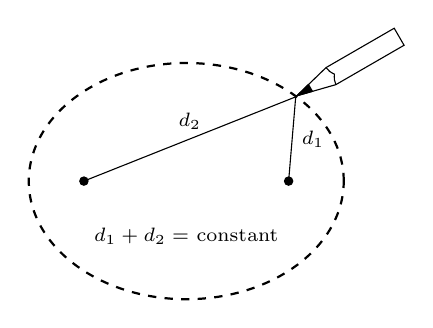
\begin{tikzpicture}
	
	\draw [thick,dashed] (0,0) circle [x radius=2,y radius=1.5];
	\filldraw (1.3,0) circle (1.5pt)
						(-1.3,0) circle (1.5pt);
	
	\draw  (1.3,0) -- node [right,pos=.5] {\scriptsize $d_1$} (1.39,1.07) -- node [above,pos=.5] {\scriptsize $d_2$} (-1.3,0);
	\draw (0,-.7) node {\scriptsize $d_1+d_2=$ constant};
	
	\begin{scope}[shift={(1.9cm,1.225cm)}]
	\begin{scope}[rotate=120]
	\begin{scope}[xscale=.25,yscale=.5]
	
	\draw (0,0) -- (0,-2) -- (1,-2)--(1,0) -- (.5,1) -- cycle;
	\draw [fill=black] (.3,.6) -- ( .5,1)--(.7,.6)--cycle;
	
	\draw (0,0) cos (.5,-.1) sin (1,0);
	
	
	\end{scope}
	\end{scope}
	\end{scope}
\end{tikzpicture}
